% ARCHITECTURE_MODERN.tex — Architecture of the Modernized SDL2 XBoing Codebase
%
% Revision history at end of front matter.
% Intended audience: contributors understanding the current architecture,
% and researchers comparing legacy vs. modern architecture for an
% AI-assisted modernization study.

\documentclass[11pt,a4paper]{article}

% --- Packages ---------------------------------------------------------------
\usepackage[utf8]{inputenc}
\usepackage[T1]{fontenc}
\usepackage{microtype}
\usepackage[margin=2.5cm]{geometry}
\usepackage{booktabs, tabularx, longtable}
\usepackage{tikz}
\usetikzlibrary{arrows.meta, positioning, shapes.geometric, calc, fit, backgrounds}
\usepackage{amsmath}
\usepackage[colorlinks=true, linkcolor=blue!70!black, urlcolor=blue!70!black, citecolor=blue!70!black]{hyperref}
\usepackage{cleveref}
\usepackage{enumitem}
\usepackage{listings}
\usepackage{xcolor}
\usepackage{parskip}

% --- Custom commands ---------------------------------------------------------
\newcommand{\adref}[1]{ADR-#1}
\newcommand{\code}[1]{\texttt{#1}}
\newcommand{\modulename}[1]{\texttt{#1}}
\newcommand{\filename}[1]{\texttt{#1}}
\newcommand{\funcname}[1]{\texttt{#1}}
\newcommand{\structname}[1]{\texttt{#1}}
\newcommand{\enumname}[1]{\texttt{#1}}
\newcommand{\legacy}{\emph{legacy}}
\newcommand{\modern}{\emph{modern}}

% --- Listings style ----------------------------------------------------------
\lstdefinestyle{cstyle}{
    language=C,
    basicstyle=\ttfamily\small,
    keywordstyle=\color{blue!70!black}\bfseries,
    commentstyle=\color{green!50!black},
    stringstyle=\color{red!60!black},
    numbers=left,
    numberstyle=\tiny\color{gray},
    numbersep=5pt,
    frame=single,
    breaklines=true,
    columns=fullflexible,
    tabsize=4,
    showstringspaces=false,
}
\lstset{style=cstyle}

% --- Title -------------------------------------------------------------------
\title{%
    \textbf{XBoing Modernized Architecture}\\[0.5em]
    \large SDL2-Based Codebase Architecture Document\\
    \large For AI-Assisted Legacy Modernization Research
}
\author{XBoing Modernization Project}
\date{March 2026 — Revision 1.0}

\begin{document}
\maketitle

% --- Revision History --------------------------------------------------------
\begin{table}[h]
\centering
\caption{Revision History}
\label{tab:revisions}
\begin{tabularx}{\textwidth}{llX}
\toprule
\textbf{Rev} & \textbf{Date} & \textbf{Description} \\
\midrule
1.0 & 2026-03-24 & Initial architecture document covering completed modernization \\
\bottomrule
\end{tabularx}
\end{table}

\tableofcontents
\newpage

% =============================================================================
\section{Introduction}
\label{sec:introduction}
% =============================================================================

XBoing is a breakout/blockout game originally written by Justin C.\ Kibell in 1993--1996 for X11 using raw Xlib, XPM pixmaps, and a fork/pipe audio architecture. The modernization replaces all platform dependencies with SDL2 while preserving the original gameplay, physics, scoring, and level format. The result is a Linux game that builds with standard SDL2 packages, follows FHS and XDG conventions, and plays identically to the original.

\subsection{Modernization Principles}
\label{sec:principles}

Five principles governed every decision:

\begin{enumerate}[nosep]
    \item \textbf{Test before you change, not after.} Characterization tests capture existing behavior before any modification.
    \item \textbf{Never rewrite from scratch.} Replace one subsystem at a time; prove equivalence with tests.
    \item \textbf{Separate concerns in commits.} A modernization commit must not also fix a bug or add a feature.
    \item \textbf{Preserve original behavior first.} Game constants (MAX\_BALLS=5, grid 18$\times$9, paddle sizes 40/50/70, DIST\_BASE=30, all scoring values) are preserved exactly.
    \item \textbf{Document architectural decisions.} All non-trivial choices are recorded as ADRs in \filename{docs/DESIGN.md} (\cref{sec:adrs}).
\end{enumerate}

\subsection{Structural Overview}
\label{sec:struct-overview}

The codebase is organized into three directories: \filename{src/*.c} (source), \filename{include/*.h} (headers), and \filename{tests/} (unit tests, integration tests, fuzz harnesses). Each source module compiles to a static library; the executable links all libraries. Three CMake presets (\code{debug}, \code{asan}, \code{install}) cover development, sanitizer, and installation builds. ADRs are recorded in \filename{docs/DESIGN.md}.


% =============================================================================
\section{Build System}
\label{sec:build-system}
% =============================================================================

CMake is the sole build system (\adref{001}). The root \filename{CMakeLists.txt} defines static library targets and 1 executable; test targets are delegated to \filename{tests/CMakeLists.txt}.

\subsection{Dependency Discovery}
\label{sec:deps}

SDL2 libraries are discovered via \code{pkg\_check\_modules}:

\begin{table}[h]
\centering
\caption{SDL2 dependencies}
\label{tab:sdl2-deps}
\begin{tabular}{lll}
\toprule
\textbf{Package} & \textbf{CMake Variable} & \textbf{Purpose} \\
\midrule
\code{sdl2} & \code{SDL2} & Window, renderer, input, timer \\
\code{SDL2\_image} & \code{SDL2\_IMAGE} & PNG texture loading \\
\code{SDL2\_mixer} & \code{SDL2\_MIXER} & WAV audio playback \\
\code{SDL2\_ttf} & \code{SDL2\_TTF} & TTF font rendering \\
\code{cmocka} & \code{CMOCKA} & Unit test framework \\
\bottomrule
\end{tabular}
\end{table}

\subsection{Library Targets}
\label{sec:lib-targets}

Each module compiles to a static library (\code{.a}). Libraries fall into five categories:

\begin{description}[nosep, leftmargin=2em]
    \item[SDL2 Platform] \modulename{sdl2\_renderer}, \modulename{sdl2\_texture}, \modulename{sdl2\_font}, \modulename{sdl2\_color}, \modulename{sdl2\_cursor}, \modulename{sdl2\_regions}, \modulename{sdl2\_audio}, \modulename{sdl2\_input}
    \item[Pure C Engine] \modulename{sdl2\_state}, \modulename{sdl2\_loop}, \modulename{sdl2\_cli}, \modulename{score\_logic}
    \item[Game Systems] \modulename{ball\_system}, \modulename{block\_system}, \modulename{paddle\_system}, \modulename{gun\_system}, \modulename{score\_system}, \modulename{level\_system}, \modulename{special\_system}, \modulename{bonus\_system}, \modulename{sfx\_system}, \modulename{eyedude\_system}, \modulename{message\_system}, \modulename{editor\_system}
    \item[UI Sequencers] \modulename{presents\_system}, \modulename{intro\_system}, \modulename{demo\_system}, \modulename{keys\_system}, \modulename{dialogue\_system}, \modulename{highscore\_system}
    \item[Persistence] \modulename{highscore\_io}, \modulename{savegame\_io}, \modulename{config\_io}, \modulename{paths}
\end{description}

One executable links all libraries: \code{xboing\_sdl2}, built only when all four SDL2 packages are found.

\subsection{Compiler Warning Policy}
\label{sec:warnings}

All targets compile with \code{-Werror} and the following warning set:

\begin{lstlisting}[language={}, numbers=none, frame=none]
-Wall -Wextra -Wpedantic -Wconversion -Wshadow
-Wdouble-promotion -Wformat=2 -Wformat-overflow=2 (GCC only)
-Wnull-dereference -Wuninitialized
-Wstrict-prototypes -Wold-style-definition
\end{lstlisting}

\subsection{CMake Presets}
\label{sec:presets}

\begin{table}[h]
\centering
\caption{CMake presets (\filename{CMakePresets.json})}
\label{tab:presets}
\begin{tabularx}{\textwidth}{llX}
\toprule
\textbf{Preset} & \textbf{Build Dir} & \textbf{Configuration} \\
\midrule
\code{debug} & \code{build/} & \code{CMAKE\_BUILD\_TYPE=Debug} \\
\code{asan} & \code{build-asan/} & Debug + \code{-fsanitize=address,undefined -fno-omit-frame-pointer} \\
\code{install} & \code{build-install/} & Release, \code{CMAKE\_INSTALL\_PREFIX=/usr}, tests disabled \\
\bottomrule
\end{tabularx}
\end{table}

\subsection{FHS Install Layout}
\label{sec:fhs}

The \code{install} preset (\adref{003}) produces an FHS-compliant installation:

\begin{lstlisting}[language={}, numbers=none, frame=none]
/usr/bin/xboing_sdl2
/usr/share/xboing/levels/*.data
/usr/share/xboing/sounds/*.wav
/usr/share/xboing/fonts/*.ttf
/usr/share/man/man6/xboing.6
/usr/share/applications/xboing.desktop
/usr/share/metainfo/com.github.xboing.metainfo.xml
/usr/share/icons/hicolor/{16,32,48,128,256}x.../xboing.png
\end{lstlisting}


% =============================================================================
\section{Architecture Overview}
\label{sec:arch-overview}
% =============================================================================

The modern codebase is organized in three layers. The SDL2 platform layer manages hardware interaction. Pure-C system libraries implement game logic with zero platform dependency. The integration layer (\filename{game\_*.c} files) wires the two together through the central \structname{game\_ctx\_t} struct.

\begin{figure}[h]
\centering
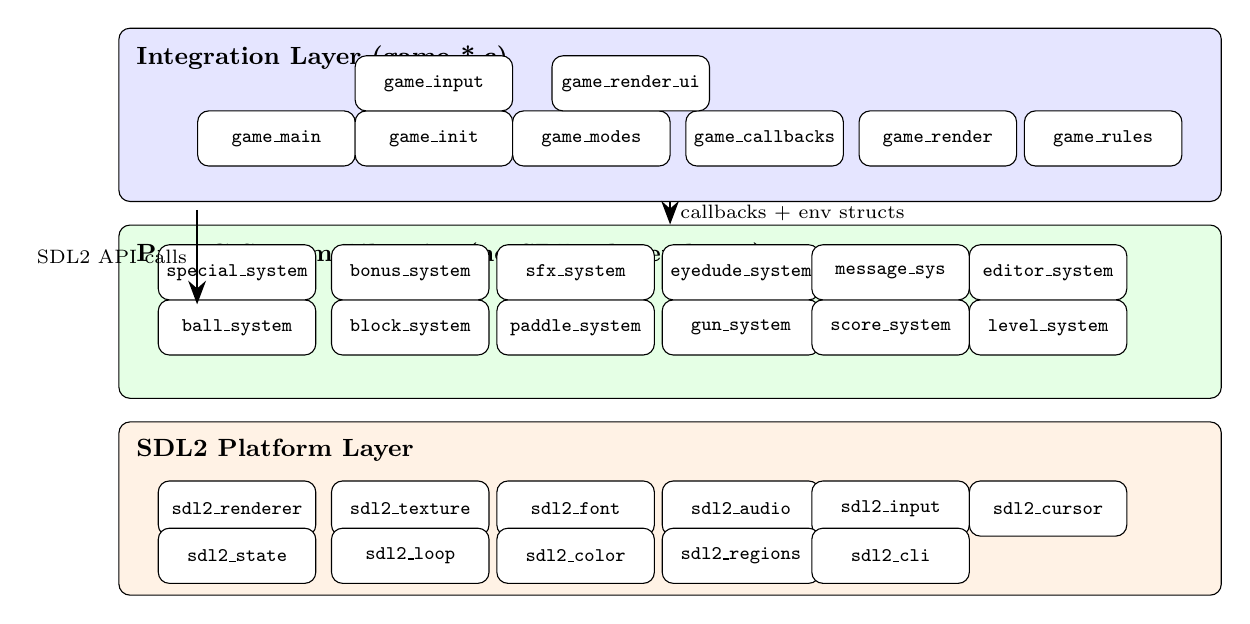
\begin{tikzpicture}[
    layer/.style={draw, rounded corners, minimum width=14cm, minimum height=2.2cm, align=center, font=\small},
    module/.style={draw, rounded corners, fill=white, minimum width=2cm, minimum height=0.7cm, font=\scriptsize\ttfamily, inner sep=2pt},
    arrow/.style={-{Stealth[length=3mm]}, thick},
    >=Stealth
]

% Integration layer (top)
\node[layer, fill=blue!10] (integration) at (0, 4.5) {};
\node[font=\small\bfseries, anchor=north west] at ([xshift=3pt, yshift=-3pt] integration.north west) {Integration Layer (game\_*.c)};
\node[module] at (-5, 4.2) {game\_main};
\node[module] at (-3, 4.2) {game\_init};
\node[module] at (-1, 4.2) {game\_modes};
\node[module] at (1.2, 4.2) {game\_callbacks};
\node[module] at (3.4, 4.2) {game\_render};
\node[module] at (5.5, 4.2) {game\_rules};
\node[module] at (-3, 4.9) {game\_input};
\node[module] at (-0.5, 4.9) {game\_render\_ui};

% Pure-C systems (middle)
\node[layer, fill=green!10] (systems) at (0, 2) {};
\node[font=\small\bfseries, anchor=north west] at ([xshift=3pt, yshift=-3pt] systems.north west) {Pure-C System Libraries (no SDL2 dependency)};
\node[module] at (-5.5, 1.8) {ball\_system};
\node[module] at (-3.3, 1.8) {block\_system};
\node[module] at (-1.2, 1.8) {paddle\_system};
\node[module] at (0.9, 1.8) {gun\_system};
\node[module] at (2.8, 1.8) {score\_system};
\node[module] at (4.8, 1.8) {level\_system};
\node[module] at (-5.5, 2.5) {special\_system};
\node[module] at (-3.3, 2.5) {bonus\_system};
\node[module] at (-1.2, 2.5) {sfx\_system};
\node[module] at (0.9, 2.5) {eyedude\_system};
\node[module] at (2.8, 2.5) {message\_sys};
\node[module] at (4.8, 2.5) {editor\_system};

% SDL2 platform (bottom)
\node[layer, fill=orange!10] (platform) at (0, -0.5) {};
\node[font=\small\bfseries, anchor=north west] at ([xshift=3pt, yshift=-3pt] platform.north west) {SDL2 Platform Layer};
\node[module] at (-5.5, -0.5) {sdl2\_renderer};
\node[module] at (-3.3, -0.5) {sdl2\_texture};
\node[module] at (-1.2, -0.5) {sdl2\_font};
\node[module] at (0.9, -0.5) {sdl2\_audio};
\node[module] at (2.8, -0.5) {sdl2\_input};
\node[module] at (4.8, -0.5) {sdl2\_cursor};
\node[module] at (-5.5, -1.1) {sdl2\_state};
\node[module] at (-3.3, -1.1) {sdl2\_loop};
\node[module] at (-1.2, -1.1) {sdl2\_color};
\node[module] at (0.9, -1.1) {sdl2\_regions};
\node[module] at (2.8, -1.1) {sdl2\_cli};

% Arrows
\draw[arrow] (integration.south) -- (systems.north) node[midway, right, font=\scriptsize] {callbacks + env structs};
\draw[arrow] (integration.south west) ++(1,-0.1) -- ++(0, -1.2) node[midway, left, font=\scriptsize] {SDL2 API calls};

\end{tikzpicture}
\caption{Three-layer architecture. Pure-C systems never call SDL2 functions; they communicate side effects through injected callback tables. The integration layer bridges both.}
\label{fig:three-layer}
\end{figure}

The defining architectural choice is \textbf{callback injection}: pure-C system libraries accept function pointer tables at creation time and invoke them for side effects (sound, score changes, block hits). The integration layer provides callback implementations that route to other systems or to SDL2 platform modules. This eliminates the 50+ \code{extern} globals that coupled legacy modules.


% =============================================================================
\section{SDL2 Platform Layer}
\label{sec:sdl2-platform}
% =============================================================================

Each SDL2 platform module follows the opaque context pattern: a heap-allocated struct hidden behind an opaque typedef, accessed only through public API functions.

\subsection{Renderer (\modulename{sdl2\_renderer})}
\label{sec:renderer}

Manages the SDL2 window and GPU-accelerated renderer (\adref{004}).

\begin{table}[h]
\centering
\caption{Renderer configuration}
\label{tab:renderer-config}
\begin{tabular}{ll}
\toprule
\textbf{Parameter} & \textbf{Value} \\
\midrule
Logical resolution & 575$\times$720 pixels \\
Default scale & 2$\times$ (physical 1150$\times$1440) \\
Window flags & \code{SDL\_WINDOW\_SHOWN | SDL\_WINDOW\_RESIZABLE} \\
Fullscreen mode & \code{SDL\_WINDOW\_FULLSCREEN\_DESKTOP} (toggle via F11) \\
Scaling filter & \code{SDL\_HINT\_RENDER\_SCALE\_QUALITY = "nearest"} \\
VSync & Enabled by default (\code{SDL\_RENDERER\_PRESENTVSYNC}) \\
Fallback & Software renderer if GPU acceleration unavailable \\
\bottomrule
\end{tabular}
\end{table}

The 575$\times$720 logical resolution matches the legacy \code{mainWindow} dimensions exactly: \code{PLAY\_WIDTH (495) + MAIN\_WIDTH (70) + 10} by \code{PLAY\_HEIGHT (580) + MAIN\_HEIGHT (130) + 10}. \code{SDL\_RenderSetLogicalSize()} handles letterboxing.

\subsection{Texture Cache (\modulename{sdl2\_texture})}
\label{sec:texture}

Loads all PNG assets into an FNV-1a hash map for O(1) lookup by string key (\adref{005}).

\begin{itemize}[nosep]
    \item \textbf{Hash map:} 256 slots, open addressing with linear probing, $\sim$70\% load factor for $\sim$180 textures.
    \item \textbf{Keys:} Relative path with \code{.png} stripped (e.g., \code{"balls/ball1"}).
    \item \textbf{Loading:} Eager---all PNGs loaded at init via recursive \code{opendir()}/\code{readdir()} directory walk.
    \item \textbf{Partial load tolerance:} Individual file failures logged but do not abort cache creation.
    \item \textbf{FNV-1a parameters:} Offset basis \code{2166136261}, prime \code{16777619}.
\end{itemize}

The hash map is write-once at initialization and read-many per frame.

\subsection{Font System (\modulename{sdl2\_font})}
\label{sec:font}

Replaces four XLFD bitmap fonts with Liberation Sans TTF via SDL2\_TTF (\adref{006}).

\begin{table}[h]
\centering
\caption{Font slots matching legacy fonts}
\label{tab:fonts}
\begin{tabular}{llrl}
\toprule
\textbf{Enum} & \textbf{Legacy XLFD} & \textbf{Size} & \textbf{Style} \\
\midrule
\code{SDL2F\_TITLE} & \code{adobe-helvetica-bold-24} & 24pt & Bold \\
\code{SDL2F\_TEXT} & \code{adobe-helvetica-medium-18} & 18pt & Regular \\
\code{SDL2F\_DATA} & \code{adobe-helvetica-bold-14} & 14pt & Bold \\
\code{SDL2F\_COPY} & \code{adobe-helvetica-medium-12} & 12pt & Regular \\
\bottomrule
\end{tabular}
\end{table}

Text rendering uses the transient texture pattern: \code{TTF\_RenderUTF8\_Blended()} $\rightarrow$ \code{SDL\_CreateTextureFromSurface()} $\rightarrow$ \code{SDL\_RenderCopy()} $\rightarrow$ destroy. Shadow text renders at $(x+2, y+2)$ in black, then $(x, y)$ in the foreground color. At $\sim$20 text draws per frame, the overhead is negligible.

\subsection{Color System (\modulename{sdl2\_color})}
\label{sec:color}

Provides precomputed RGBA values verified against X11 \filename{rgb.txt} (\adref{007}). Unlike other SDL2 modules, this has \textbf{no opaque context}---all data is \code{static const}.

\begin{itemize}[nosep]
    \item 8 named colors: RED, TAN, YELLOW, GREEN, WHITE, BLACK, BLUE, PURPLE.
    \item 2 gradient arrays: \code{sdl2\_color\_red\_gradient(i)} and \code{sdl2\_color\_green\_gradient(i)}, each 7 steps, matching legacy hex values (\code{\#f00} through \code{\#300}).
    \item String lookup via \code{sdl2\_color\_by\_name()} for migration from \code{ColourNameToPixel()} call sites.
\end{itemize}

\subsection{Cursor Management (\modulename{sdl2\_cursor})}
\label{sec:cursor}

Pre-creates 5 cursor types at init (\adref{008}), switching via O(1) \code{SDL\_SetCursor()}:

\begin{table}[h]
\centering
\caption{Cursor mapping from legacy to SDL2}
\label{tab:cursors}
\begin{tabular}{lll}
\toprule
\textbf{Enum} & \textbf{Legacy X11} & \textbf{SDL2 System Cursor} \\
\midrule
\code{SDL2CUR\_WAIT} & \code{XC\_watch} & \code{SDL\_SYSTEM\_CURSOR\_WAIT} \\
\code{SDL2CUR\_PLUS} & \code{XC\_plus} & \code{SDL\_SYSTEM\_CURSOR\_CROSSHAIR} \\
\code{SDL2CUR\_POINT} & \code{XC\_hand2} & \code{SDL\_SYSTEM\_CURSOR\_HAND} \\
\code{SDL2CUR\_SKULL} & \code{XC\_pirate} & \code{SDL\_SYSTEM\_CURSOR\_CROSSHAIR} \\
\code{SDL2CUR\_NONE} & blank pixmap & \code{SDL\_ShowCursor(SDL\_DISABLE)} \\
\bottomrule
\end{tabular}
\end{table}

Best-effort creation: missing cursors (e.g., dummy driver) are stored as NULL; \code{set()} gracefully skips \code{SDL\_SetCursor} while still tracking the active cursor ID.

\subsection{Logical Regions (\modulename{sdl2\_regions})}
\label{sec:regions}

Replaces 10 X11 sub-windows with 9 named \code{SDL\_Rect} constants in the 575$\times$720 logical coordinate system (\adref{009}). No opaque context---pure static data.

\begin{table}[h]
\centering
\caption{Logical render regions (all coordinates in pixels)}
\label{tab:regions}
\begin{tabular}{lrrrr}
\toprule
\textbf{Region} & \textbf{X} & \textbf{Y} & \textbf{W} & \textbf{H} \\
\midrule
PLAY & 35 & 60 & 495 & 580 \\
SCORE & 35 & 10 & 224 & 42 \\
LEVEL & 284 & 5 & 286 & 52 \\
MESSAGE & 35 & 655 & 247 & 30 \\
SPECIAL & 292 & 655 & 180 & 35 \\
TIMER & 477 & 655 & 61 & 35 \\
EDITOR & \multicolumn{4}{l}{Editor-specific block palette} \\
EDITOR\_TYPE & \multicolumn{4}{l}{Editor-specific type display} \\
DIALOGUE & \multicolumn{4}{l}{Centered modal input overlay} \\
\bottomrule
\end{tabular}
\end{table}

Hit testing via \funcname{sdl2\_region\_hit\_test(x, y)} maps pixel coordinates to region IDs for mouse dispatch.

\subsection{Audio (\modulename{sdl2\_audio})}
\label{sec:audio}

Replaces the fork/pipe architecture and 12 platform-specific drivers with SDL2\_mixer (\adref{010}).

\begin{itemize}[nosep]
    \item \textbf{Eager WAV caching:} Scans sound directory at init, loads all \code{.wav} files into an FNV-1a hash map keyed by basename (e.g., \code{"boing"}).
    \item \textbf{Concurrent playback:} \code{Mix\_PlayChannel(-1, chunk, 0)} auto-selects from 16 allocated channels. Legacy could only play one sound at a time.
    \item \textbf{Global volume:} \code{Mix\_Volume(-1, vol)} applies to all channels.
    \item \textbf{CI testing:} \code{SDL\_AUDIODRIVER=dummy} enables headless operation.
\end{itemize}

\subsection{Input Mapping (\modulename{sdl2\_input})}
\label{sec:input}

Replaces \code{XLookupString()} KeySym dispatch with a scancode-to-action mapping layer (\adref{011}).

\begin{itemize}[nosep]
    \item Game actions covering movement, gameplay, menu, global controls, and 9 speed levels (see \enumname{sdl2\_input\_action\_t}).
    \item Dual binding slots per action (e.g., Left arrow + J for paddle left).
    \item O(1) reverse lookup table: \code{SDL\_Scancode $\rightarrow$ action} array (\code{SDL\_NUM\_SCANCODES} entries).
    \item Level trigger (\code{pressed()}) for held keys; edge trigger (\code{just\_pressed()}) for one-shot actions.
    \item Mouse position and button state from \code{SDL\_MOUSEMOTION}/\code{SDL\_MOUSEBUTTONDOWN}.
    \item Runtime rebindable via \code{bind()}/\code{reset\_bindings()}.
\end{itemize}

\subsection{State Machine Engine (\modulename{sdl2\_state})}
\label{sec:state-machine}

Replaces the legacy \code{switch(mode)} dispatch with a function pointer table (\adref{012}). Pure C---no SDL2 dependency.

\begin{table}[h]
\centering
\caption{Game modes (16 values matching legacy \code{MODE\_*} defines)}
\label{tab:modes}
\begin{tabular}{rl}
\toprule
\textbf{Value} & \textbf{Mode} \\
\midrule
0 & NONE \\
1 & HIGHSCORE \\
2 & INTRO \\
3 & GAME \\
4 & PAUSE \\
5 & BALL\_WAIT (legacy: never assigned) \\
6 & WAIT (legacy: never assigned) \\
7 & BONUS \\
8 & INSTRUCT \\
9 & KEYS \\
10 & PRESENTS \\
11 & DEMO \\
12 & PREVIEW \\
13 & DIALOGUE \\
14 & EDIT \\
15 & KEYSEDIT \\
\bottomrule
\end{tabular}
\end{table}

Each mode registers three optional callbacks via \structname{sdl2\_state\_mode\_def\_t}:
\code{on\_enter}, \code{on\_update}, \code{on\_exit}. Transitions call exit on the old mode, then enter on the new. Dialogue mode uses push/pop semantics (\funcname{push\_dialogue()}/\funcname{pop\_dialogue()}) to save and restore the interrupted mode.

The frame counter increments on every \funcname{update()} except in PAUSE and DIALOGUE modes.

\subsection{Game Loop (\modulename{sdl2\_loop})}
\label{sec:game-loop}

Fixed-timestep accumulator replacing legacy \code{usleep()} timing (\adref{013}). Pure C---no SDL2 dependency.

\begin{figure}[h]
\centering
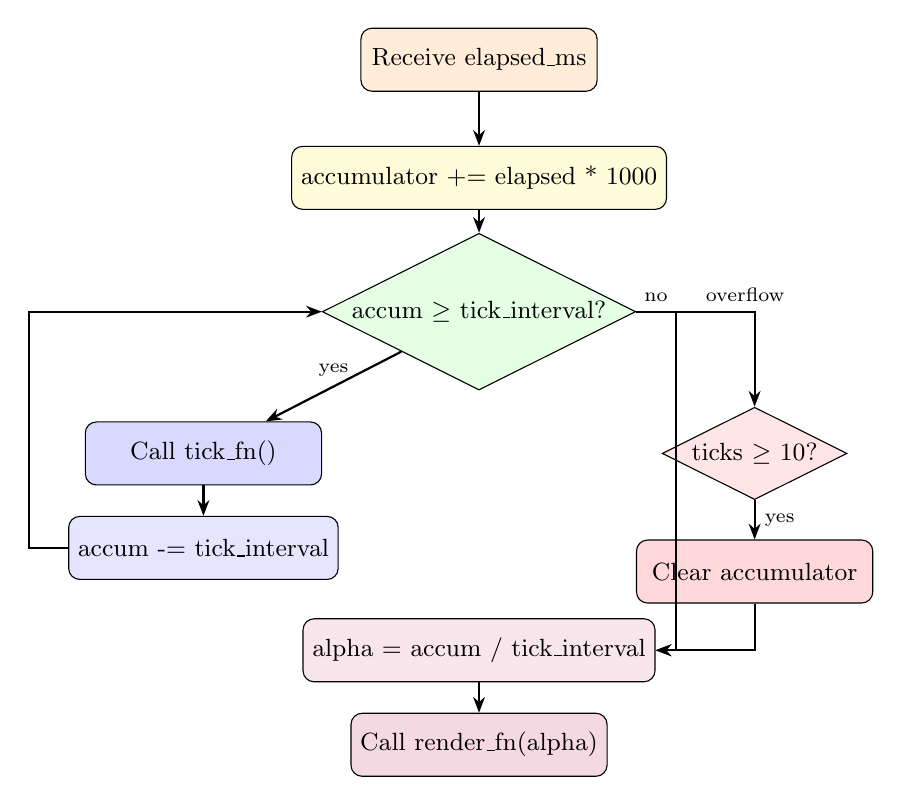
\begin{tikzpicture}[
    box/.style={draw, rounded corners, minimum width=3cm, minimum height=0.8cm, font=\small},
    decision/.style={draw, diamond, aspect=2, font=\small, inner sep=1pt},
    arrow/.style={-{Stealth[length=2mm]}, thick},
]
\node[box, fill=orange!15] (elapsed) at (0,0) {Receive elapsed\_ms};
\node[box, fill=yellow!15] (accum) at (0,-1.5) {accumulator += elapsed * 1000};
\node[decision, fill=green!10] (check) at (0,-3.2) {accum $\geq$ tick\_interval?};
\node[box, fill=blue!15] (tick) at (-3.5,-5) {Call tick\_fn()};
\node[box, fill=blue!10] (sub) at (-3.5,-6.2) {accum -= tick\_interval};
\node[decision, fill=red!10] (cap) at (3.5,-5) {ticks $\geq$ 10?};
\node[box, fill=red!15] (clear) at (3.5,-6.5) {Clear accumulator};
\node[box, fill=purple!10] (alpha) at (0,-7.5) {alpha = accum / tick\_interval};
\node[box, fill=purple!15] (render) at (0,-8.7) {Call render\_fn(alpha)};

\draw[arrow] (elapsed) -- (accum);
\draw[arrow] (accum) -- (check);
\draw[arrow] (check) -- node[above, font=\scriptsize]{yes} (tick);
\draw[arrow] (tick) -- (sub);
\draw[arrow] (sub.west) -- ++(-0.5,0) |- (check.west);
\draw[arrow] (check) -- node[above, font=\scriptsize]{no} ++(2.5,0) |- (alpha);
\draw[arrow] (check) -| node[above right, font=\scriptsize, pos=0.25]{overflow} (cap);
\draw[arrow] (cap) -- node[right, font=\scriptsize]{yes} (clear);
\draw[arrow] (clear.south) |- (alpha);
\draw[arrow] (alpha) -- (render);

\end{tikzpicture}
\caption{Fixed-timestep game loop. Tick interval = $1500 \times (10 - \text{speed\_level})$ microseconds. Spiral-of-death prevention caps at 10 ticks per frame.}
\label{fig:game-loop}
\end{figure}

\begin{table}[h]
\centering
\caption{Speed level tick rates}
\label{tab:speed-levels}
\begin{tabular}{rrr}
\toprule
\textbf{Speed} & \textbf{Tick Interval} & \textbf{Ticks/sec} \\
\midrule
1 (slowest) & 13{,}500 $\mu$s & $\sim$74 \\
5 (default) & 7{,}500 $\mu$s & $\sim$133 \\
9 (fastest) & 1{,}500 $\mu$s & $\sim$667 \\
\bottomrule
\end{tabular}
\end{table}

\subsection{CLI Parser (\modulename{sdl2\_cli})}
\label{sec:cli}

Pure C command-line parser (\adref{014}). Populates a \structname{sdl2\_cli\_config\_t} struct with no side effects. Legacy X11-specific options (\code{-display}, \code{-geometry}, etc.) are dropped. Status codes distinguish informational exits (\code{EXIT\_HELP}, \code{EXIT\_VERSION}) from errors (\code{ERR\_MISSING\_VALUE}, \code{ERR\_INVALID\_VALUE}).


% =============================================================================
\section{Pure-C System Libraries}
\label{sec:systems}
% =============================================================================

All game system modules share these properties:
\begin{enumerate}[nosep]
    \item \textbf{Opaque context:} Heap-allocated via \code{calloc()}, destroyed via \code{free()}. No global or static mutable state.
    \item \textbf{Callback injection:} Side effects communicated through function pointer tables provided at creation. Any callback may be NULL (no-op).
    \item \textbf{Environment structs:} Per-frame state from other systems passed as const structs, never cached.
    \item \textbf{No SDL2 or X11 dependency:} Links only \code{libc} (and \code{libm} for ball physics).
    \item \textbf{Render info queries:} Position, animation frame, and visibility data returned through caller-provided structs. The system never renders.
\end{enumerate}

\subsection{Ball System (\modulename{ball\_system})}
\label{sec:ball-system}

Owns the \code{BALL} array (up to \code{MAX\_BALLS}=5), state machine dispatch, physics, and queries (\adref{015}).

\textbf{State machine per ball:} \code{BALL\_CREATE} $\rightarrow$ \code{BALL\_READY} (sitting on paddle) $\rightarrow$ \code{BALL\_ACTIVE} (in play) $\rightarrow$ \code{BALL\_POP} (death animation) $\rightarrow$ \code{BALL\_NONE} (slot freed).

\textbf{Environment struct} (\structname{ball\_system\_env\_t}) carries 12 values replacing legacy extern globals:

\begin{lstlisting}[language=C, numbers=none, frame=none]
typedef struct {
    int frame, speed_level, paddle_pos, paddle_dx, paddle_size;
    int play_width, play_height;   /* 495, 580 */
    int no_walls, killer, sticky_bat;
    int col_width, row_height;     /* 55, 32 */
} ball_system_env_t;
\end{lstlisting}

\textbf{Callback table} (7 function pointers):
\begin{description}[nosep, leftmargin=2em, font=\ttfamily\small]
    \item[check\_region] Block collision check (replaces \code{XRectInRegion()})
    \item[on\_block\_hit] Block hit dispatch (replaces \code{HandleTheBlocks()})
    \item[cell\_available] Grid query for hyperspace teleport
    \item[on\_sound] Sound effect playback
    \item[on\_score] Point award
    \item[on\_message] Status bar update
    \item[on\_event] Lifecycle events (died, split, tilt, paddle hit)
\end{description}

Physics functions are extracted to \filename{ball\_math.c}: paddle bounce (trigonometric angle calculation), speed normalization, ball-to-ball elastic collision.

\subsection{Block System (\modulename{block\_system})}
\label{sec:block-system}

Owns the 18$\times$9 block grid with pure-C diagonal cross-product collision replacing X11 Regions (\adref{016}).

\textbf{Collision algorithm:} The block rectangle is divided into 4 triangles by its diagonals. Two cross-product values determine the hit face:

\begin{align}
d_1 &= w \cdot (b_y - y) - h \cdot (b_x - x) & \text{(TL--BR diagonal)} \label{eq:d1} \\
d_2 &= h \cdot (x + w - b_x) - w \cdot (b_y - y) & \text{(TR--BL diagonal)} \label{eq:d2}
\end{align}

\begin{table}[h]
\centering
\caption{Cross-product region classification}
\label{tab:cross-product}
\begin{tabular}{ccl}
\toprule
$d_1$ & $d_2$ & \textbf{Hit Face} \\
\midrule
$\leq 0$ & $\geq 0$ & TOP \\
$\geq 0$ & $\leq 0$ & BOTTOM \\
$\geq 0$ & $\geq 0$ & LEFT \\
$\leq 0$ & $\leq 0$ & RIGHT \\
\bottomrule
\end{tabular}
\end{table}

Three-step collision check: (1) AABB overlap test, (2) diagonal cross-product for hit face, (3) adjacency filter suppresses bounce if neighbor in that direction is occupied.

The block info catalog stores metadata for all 30 block types (point values, animation frames, explode behavior).

\subsection{Paddle System (\modulename{paddle\_system})}
\label{sec:paddle-system}

Owns paddle position, size (3 sizes: 40/50/70 pixels), and control flags (\adref{017}). Keyboard mode applies \code{PADDLE\_VELOCITY}=4 per frame. Mouse mode uses the legacy formula: \code{pos = mouse\_x - (main\_width / 2) + half\_width}. Reverse controls swap keyboard direction and mirror mouse X.

\subsection{Gun System (\modulename{gun\_system})}
\label{sec:gun-system}

Owns bullet (40 slots) and tink (40 slots) arrays, ammo state, movement physics, and collision dispatch (\adref{018}). Normal mode uses slot 0 only; fast gun mode searches all 40 slots, spawning 2 bullets per shot. Collision priority: ball $>$ eyedude $>$ block.

\subsection{Score System (\modulename{score\_system})}
\label{sec:score-system}

Owns score value, multiplier application, extra life tracking (every 100{,}000 points), and digit layout computation (\adref{019}). Delegates arithmetic to \modulename{score\_logic}: \funcname{score\_apply\_multiplier()}, \funcname{score\_extra\_life\_threshold()}, \funcname{score\_block\_hit\_points()}. The x2-wins-over-x4 legacy bug is preserved.

Digit layout: right-aligned, rightmost digit at x=192 (224$-$32), stride 32px, max 7 digits (9{,}999{,}999).

\subsection{Level System (\modulename{level\_system})}
\label{sec:level-system}

Parses level data files (title, time bonus, 15$\times$9 character grid) and fires \code{on\_add\_block(row, col, type, counter\_slide)} for each cell (\adref{020}). 30 distinct characters map to block types. 80 levels cycle via \code{level \% 80} (mapping 0 to 80). Background cycling: 2$\rightarrow$3$\rightarrow$4$\rightarrow$5$\rightarrow$2.

\subsection{Special System (\modulename{special\_system})}
\label{sec:special-system}

Owns 8 power-up flags (\adref{021}): reverse (display only, owned by paddle system), sticky, saving, fastGun, noWalls, killer, x2, x4. Setting x2 deactivates x4 and vice versa. \funcname{turn\_off()} clears all except saving (legacy intentional behavior). \funcname{get\_labels()} returns render info for the 4$\times$2 panel display.

\subsection{Bonus System (\modulename{bonus\_system})}
\label{sec:bonus-system}

10-state tally sequence after level completion (\adref{022}). Score is pre-committed at sequence entry (animated tally is cosmetic). Save triggers every \code{SAVE\_LEVEL}=5 levels relative to starting level. Pure functions \funcname{compute\_total()} and \funcname{should\_save()} are independently testable.

\subsection{SFX System (\modulename{sfx\_system})}
\label{sec:sfx-system}

5 visual effects (SHAKE, FADE, BLIND, SHATTER, STATIC) plus BorderGlow ambient animation (\adref{023}). No rendering---query functions return coordinates and tile data. SHAKE uses \code{on\_move\_window} callback. BorderGlow cycles 7-step red/green ramps on 40-frame intervals. STATIC is preserved as the original stub.

\subsection{EyeDude System (\modulename{eyedude\_system})}
\label{sec:eyedude-system}

Animated character with 6 walk frames per direction, random direction, turn-at-midpoint, AABB collision detection (\adref{024}). Awards 10{,}000 points on ball hit. Constants: WIDTH=32, HEIGHT=32, FRAME\_RATE=30, WALK\_SPEED=5, TURN\_CHANCE=30\%.

\subsection{Message System (\modulename{message\_system})}
\label{sec:message-system}

Single-line message bar with optional auto-clear delay. Reverts to default message (level title) when delay expires.

\subsection{Editor System (\modulename{editor\_system})}
\label{sec:editor-system}

Grid editing (draw/erase), board transforms (flip/scroll H/V), palette management, save/load via callbacks. Play-test transitions preserve editor state for return.

\subsection{UI Sequencers}
\label{sec:ui-sequencers}

Six UI sequencer modules implement attract-mode and post-game screens. All follow the sequencer pattern: advance state per frame, expose query functions for render data, fire callbacks for sound and external events.

\begin{table}[h]
\centering
\caption{UI sequencer modules}
\label{tab:ui-sequencers}
\begin{tabularx}{\textwidth}{llX}
\toprule
\textbf{Module} & \textbf{ADR} & \textbf{States / Purpose} \\
\midrule
\modulename{presents\_system} & \adref{025} & 14 states: flag, credits, letter stamps, sparkle, typewriter text, curtain wipe \\
\modulename{intro\_system} & \adref{026} & 2 modes (intro + instructions), block descriptions table, sparkle \\
\modulename{demo\_system} & \adref{027} & 2 modes (demo + preview), ball trail data, random level loading \\
\modulename{keys\_system} & \adref{028} & 2 modes (game + editor controls), static key binding tables \\
\modulename{dialogue\_system} & --- & 4 validation modes (text, numeric, printable, yes/no), input buffer \\
\modulename{highscore\_system} & --- & Title sparkle, row sparkle, specials timing, score display \\
\bottomrule
\end{tabularx}
\end{table}

The attract mode cycle runs: PRESENTS $\rightarrow$ INTRO $\rightarrow$ INSTRUCT $\rightarrow$ DEMO $\rightarrow$ KEYS $\rightarrow$ KEYSEDIT $\rightarrow$ PREVIEW $\rightarrow$ HIGHSCORE $\rightarrow$ INTRO (loops).


% =============================================================================
\section{Integration Layer}
\label{sec:integration}
% =============================================================================

Eight source files in \filename{src/game\_*.c} wire the platform and system layers together. None are compiled as libraries; they are compiled directly into the \code{xboing\_sdl2} executable.

\subsection{Game Context (\structname{game\_ctx\_t})}
\label{sec:game-context}

The central struct (\filename{include/game\_context.h}) holds pointers to all module contexts plus shared game state. It is passed as \code{void *user\_data} to every callback.

\begin{figure}[h]
\centering
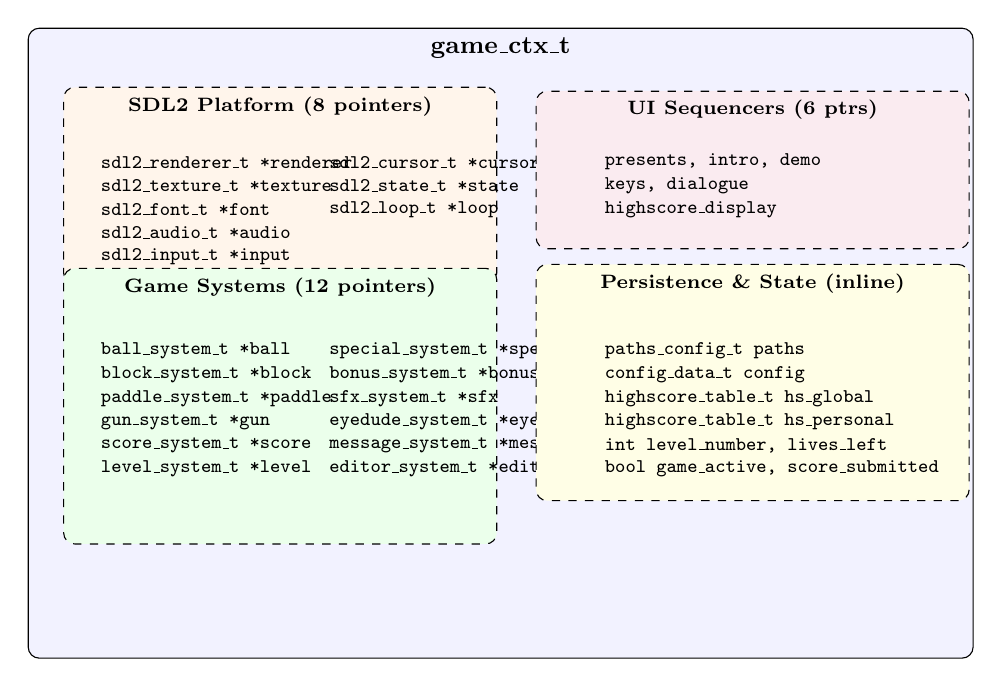
\begin{tikzpicture}[
    ctx/.style={draw, rounded corners, fill=blue!5, minimum width=12cm, minimum height=8cm},
    group/.style={draw, dashed, rounded corners, fill=#1, minimum width=5.5cm, inner sep=4pt},
    field/.style={font=\scriptsize\ttfamily, anchor=west},
]
\node[ctx] (ctx) at (0,0) {};
\node[font=\small\bfseries, anchor=north] at (ctx.north) {game\_ctx\_t};

% SDL2 platform group
\node[group=orange!8, minimum height=2.5cm] (sdl2) at (-2.8, 2) {};
\node[font=\scriptsize\bfseries, anchor=north] at (sdl2.north) {SDL2 Platform (8 pointers)};
\node[field] at (-5.2, 2.3) {sdl2\_renderer\_t *renderer};
\node[field] at (-5.2, 2.0) {sdl2\_texture\_t *texture};
\node[field] at (-5.2, 1.7) {sdl2\_font\_t *font};
\node[field] at (-5.2, 1.4) {sdl2\_audio\_t *audio};
\node[field] at (-5.2, 1.1) {sdl2\_input\_t *input};
\node[field] at (-2.3, 2.3) {sdl2\_cursor\_t *cursor};
\node[field] at (-2.3, 2.0) {sdl2\_state\_t *state};
\node[field] at (-2.3, 1.7) {sdl2\_loop\_t *loop};

% Game systems group
\node[group=green!8, minimum height=3.5cm] (sys) at (-2.8, -0.8) {};
\node[font=\scriptsize\bfseries, anchor=north] at (sys.north) {Game Systems (12 pointers)};
\node[field] at (-5.2, -0.1) {ball\_system\_t *ball};
\node[field] at (-5.2, -0.4) {block\_system\_t *block};
\node[field] at (-5.2, -0.7) {paddle\_system\_t *paddle};
\node[field] at (-5.2, -1.0) {gun\_system\_t *gun};
\node[field] at (-5.2, -1.3) {score\_system\_t *score};
\node[field] at (-5.2, -1.6) {level\_system\_t *level};
\node[field] at (-2.3, -0.1) {special\_system\_t *special};
\node[field] at (-2.3, -0.4) {bonus\_system\_t *bonus};
\node[field] at (-2.3, -0.7) {sfx\_system\_t *sfx};
\node[field] at (-2.3, -1.0) {eyedude\_system\_t *eyedude};
\node[field] at (-2.3, -1.3) {message\_system\_t *message};
\node[field] at (-2.3, -1.6) {editor\_system\_t *editor};

% UI sequencers + state
\node[group=purple!8, minimum height=2cm] (ui) at (3.2, 2.2) {};
\node[font=\scriptsize\bfseries, anchor=north] at (ui.north) {UI Sequencers (6 ptrs)};
\node[field] at (1.2, 2.3) {presents, intro, demo};
\node[field] at (1.2, 2.0) {keys, dialogue};
\node[field] at (1.2, 1.7) {highscore\_display};

% Persistence + game state
\node[group=yellow!10, minimum height=3cm] (state) at (3.2, -0.5) {};
\node[font=\scriptsize\bfseries, anchor=north] at (state.north) {Persistence \& State (inline)};
\node[field] at (1.2, -0.1) {paths\_config\_t paths};
\node[field] at (1.2, -0.4) {config\_data\_t config};
\node[field] at (1.2, -0.7) {highscore\_table\_t hs\_global};
\node[field] at (1.2, -1.0) {highscore\_table\_t hs\_personal};
\node[field] at (1.2, -1.3) {int level\_number, lives\_left};
\node[field] at (1.2, -1.6) {bool game\_active, score\_submitted};

\end{tikzpicture}
\caption{\structname{game\_ctx\_t} composition. Pointer members reference heap-allocated opaque contexts; persistence and game state fields are owned inline.}
\label{fig:game-context}
\end{figure}

Module contexts are forward-declared as opaque typedefs in \filename{game\_context.h} to avoid header inclusion cycles. Only \filename{config\_io.h}, \filename{highscore\_system.h}, and \filename{paths.h} are included (for inline value types).

\subsection{Initialization (\filename{game\_init.c})}
\label{sec:game-init}

\funcname{game\_create(argc, argv)} builds the full context in dependency order:

\begin{enumerate}[nosep]
    \item CLI parsing + config file loading + XDG path resolution + high score table loading
    \item SDL2 initialization (\code{SDL\_Init(VIDEO|AUDIO|TIMER)})
    \item Platform modules: renderer $\rightarrow$ texture $\rightarrow$ font $\rightarrow$ audio $\rightarrow$ input $\rightarrow$ cursor
    \item State machine + game loop (with tick/render callbacks)
    \item Game systems: block $\rightarrow$ paddle $\rightarrow$ ball $\rightarrow$ gun $\rightarrow$ score $\rightarrow$ level $\rightarrow$ special $\rightarrow$ bonus $\rightarrow$ sfx $\rightarrow$ eyedude $\rightarrow$ message $\rightarrow$ editor
    \item UI sequencers: presents, intro, demo, keys, dialogue, highscore
    \item Mode handler registration with the state machine
\end{enumerate}

\funcname{game\_destroy()} tears down in reverse order.

\subsection{Callback Wiring (\filename{game\_callbacks.c})}
\label{sec:callbacks}

The callback injection pattern is the defining architectural choice. Each pure-C system library declares a callback table struct. The integration layer provides implementations that cast the \code{void *user\_data} parameter to \structname{game\_ctx\_t*} and dispatch to the appropriate module.

\begin{figure}[h]
\centering
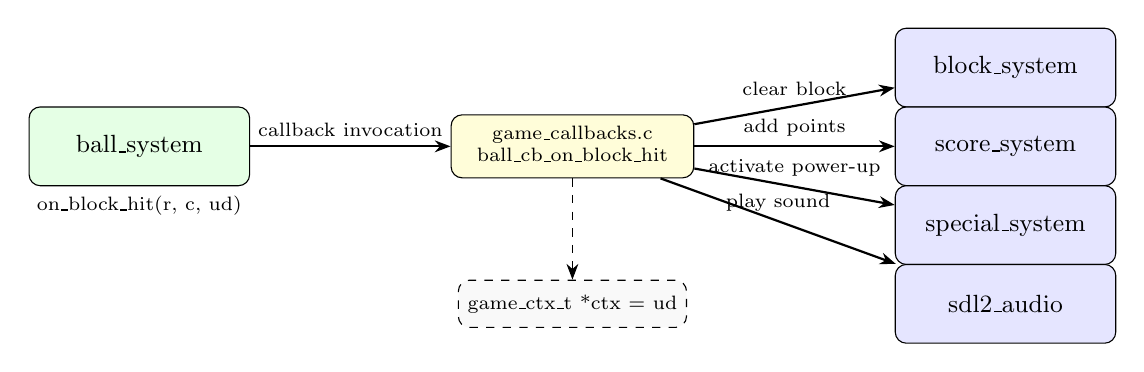
\begin{tikzpicture}[
    system/.style={draw, rounded corners, fill=green!10, minimum width=2.8cm, minimum height=1cm, font=\small},
    callback/.style={draw, rounded corners, fill=yellow!15, minimum width=3cm, minimum height=0.8cm, font=\scriptsize},
    target/.style={draw, rounded corners, fill=blue!10, minimum width=2.8cm, minimum height=1cm, font=\small},
    arrow/.style={-{Stealth[length=2mm]}, thick},
]

% Source system
\node[system] (ball) at (0, 0) {ball\_system};
\node[font=\scriptsize, below=0pt of ball] {on\_block\_hit(r, c, ud)};

% Callback in integration layer
\node[callback] (cb) at (5.5, 0) {\begin{tabular}{c}game\_callbacks.c\\ball\_cb\_on\_block\_hit\end{tabular}};

% Target systems
\node[target] (block) at (11, 1) {block\_system};
\node[target] (score) at (11, 0) {score\_system};
\node[target] (special) at (11, -1) {special\_system};
\node[target] (audio) at (11, -2) {sdl2\_audio};

% Arrows
\draw[arrow] (ball) -- (cb) node[midway, above, font=\scriptsize] {callback invocation};
\draw[arrow] (cb) -- (block) node[midway, above, font=\scriptsize] {clear block};
\draw[arrow] (cb) -- (score) node[midway, above, font=\scriptsize] {add points};
\draw[arrow] (cb) -- (special) node[midway, above, font=\scriptsize] {activate power-up};
\draw[arrow] (cb) -- (audio) node[midway, above, font=\scriptsize] {play sound};

% Context
\node[draw, dashed, rounded corners, fill=gray!5, minimum width=2cm, minimum height=0.6cm, font=\scriptsize] (ctx) at (5.5, -2) {game\_ctx\_t *ctx = ud};
\draw[-{Stealth[length=2mm]}, dashed] (cb) -- (ctx);

\end{tikzpicture}
\caption{Callback injection flow. The ball system invokes \code{on\_block\_hit} via function pointer. The integration layer casts \code{user\_data} to \structname{game\_ctx\_t*} and dispatches to multiple target systems.}
\label{fig:callback-flow}
\end{figure}

\textbf{Example: ball block hit callback} (from \filename{game\_callbacks.c}):
\begin{lstlisting}[language=C]
static int ball_cb_on_block_hit(int row, int col, int ball_index, void *ud)
{
    game_ctx_t *ctx = ud;
    int block_type = block_system_get_type(ctx->block, row, col);
    int points = score_block_hit_points(block_type, row);
    if (points > 0) {
        score_system_env_t senv = {
            .x2_active = special_system_is_active(ctx->special, SPECIAL_X2_BONUS),
            .x4_active = special_system_is_active(ctx->special, SPECIAL_X4_BONUS),
        };
        score_system_add(ctx->score, (unsigned long)points, &senv);
    }
    switch (block_type) {
        case DEATH_BLK: block_system_clear(ctx->block, row, col); return 1;
        case BOMB_BLK:  /* clear neighbors */ ...
        case MULTIBALL_BLK: ball_system_split(ctx->ball, &env); ...
        /* 15+ more block type handlers */
    }
}
\end{lstlisting}

This pattern eliminates the 50+ \code{extern} globals that coupled legacy modules. Each system library is independently testable by providing stub callbacks.

\subsection{Mode Handlers (\filename{game\_modes.c})}
\label{sec:mode-handlers}

Registers \code{on\_enter}/\code{on\_update}/\code{on\_exit} handlers for each of the 16 game modes with the state machine. Mode-specific logic includes:

\begin{description}[nosep, leftmargin=2em]
    \item[GAME] Core gameplay: updates ball, paddle, gun, eyedude, sfx, bonus spawning, timer countdown.
    \item[PAUSE] Pauses the game loop, displays pause overlay.
    \item[BONUS] Drives the 10-state bonus tally sequence, transitions to next level on completion.
    \item[PRESENTS/INTRO/DEMO/KEYS] Attract mode screens with frame-driven state machines.
    \item[EDIT] Level editor with palette, grid editing, play-test transitions.
    \item[DIALOGUE] Modal text input (name entry, level selection, ``words of wisdom'').
\end{description}

\subsection{Rendering (\filename{game\_render.c} + \filename{game\_render\_ui.c})}
\label{sec:rendering}

\filename{game\_render.c} draws gameplay elements (blocks, balls, paddle, bullets, score, lives, specials, messages, timer, border, EyeDude). \filename{game\_render\_ui.c} draws UI screens (presents, intro, demo, keys, bonus, highscore, editor, dialogue).

Each render function queries its corresponding system for render info and draws textures from the sprite catalog. The render dispatch is called once per frame with an interpolation alpha for smooth animation.

\subsection{Input Dispatch (\filename{game\_input.c})}
\label{sec:input-dispatch}

Routes input actions to the appropriate handler based on the current game mode. Gameplay mode handles paddle movement, shooting, tilt, save/load. Attract modes handle start/cycle/quit. Editor mode handles draw/erase/palette/transforms.

\subsection{Game Rules (\filename{game\_rules.c})}
\label{sec:game-rules}

Per-frame game logic: level completion detection (all breakable blocks cleared), ball death handling (decrement lives, reset ball or game over), bonus block spawning (random timing, 27 block types with probability distribution), and timer countdown (1-second decrement via frame accumulator).


% =============================================================================
\section{Persistence}
\label{sec:persistence}
% =============================================================================

Four persistence modules handle file I/O with no SDL2 dependency.

\subsection{High Score I/O (\modulename{highscore\_io})}
\label{sec:highscore-io}

JSON format replacing legacy binary \code{highScoreHeader} + \code{highScoreEntry} with \code{htonl} byte ordering. Hand-written JSON parser and emitter (no external dependency). Atomic writes via write-to-temp + rename. Two tables: global (shared) and personal (per-user).

\subsection{Save Game I/O (\modulename{savegame\_io})}
\label{sec:savegame-io}

JSON format replacing legacy binary \code{saveGameStruct}. Saves level number, score, lives, specials state, block grid snapshot. Atomic writes.

\subsection{Config I/O (\modulename{config\_io})}
\label{sec:config-io}

Minimal TOML format (flat key=value, no tables). Stores user preferences: speed, volume, nickname, sound/SFX enable, control mode. Located at \code{\$XDG\_DATA\_HOME/xboing/config.toml}. CLI flags override config file values.

\subsection{Path Resolution (\modulename{paths})}
\label{sec:paths}

XDG Base Directory path resolution (\adref{002}). Centralizes all file path logic (12+ scattered callsites in legacy).

\textbf{Read-only assets} (levels, sounds) resolution priority:
\begin{enumerate}[nosep]
    \item Legacy env var (\code{XBOING\_LEVELS\_DIR})
    \item \code{XDG\_DATA\_DIRS} search
    \item \code{XDG\_DATA\_HOME}
    \item CWD fallback (\code{./levels/})
\end{enumerate}

\textbf{Writable state} (scores, saves) resolution priority:
\begin{enumerate}[nosep]
    \item Legacy env var (\code{XBOING\_SCORE\_FILE})
    \item Existing legacy file (\code{\$HOME/.xboing-scores})
    \item XDG default (\code{\$XDG\_DATA\_HOME/xboing/scores.dat})
\end{enumerate}

Design constraint: caller-provided buffers (no malloc, no static buffers). \funcname{paths\_init\_explicit()} accepts injected env values for deterministic testing.


% =============================================================================
\section{Design Patterns}
\label{sec:patterns}
% =============================================================================

\subsection{Opaque Context Pattern}
\label{sec:opaque-context}

Every system module defines a struct visible only in the \code{.c} file and exposes an opaque typedef in the \code{.h} file via forward declaration. The integration layer holds pointers to these opaque structs in \structname{game\_ctx\_t}.

Consequences:
\begin{itemize}[nosep]
    \item Zero global mutable state across the entire modern codebase.
    \item Each module is independently testable via CMocka---create a context, inject stub callbacks, exercise API, destroy context.
    \item Header inclusion cycles are impossible: \filename{game\_context.h} uses only forward declarations.
    \item Multiple game instances could coexist (relevant for future replay comparison or headless testing).
\end{itemize}

\subsection{Callback Injection}
\label{sec:callback-injection}

System libraries never call other system libraries directly. Side effects are communicated through function pointer tables (\cref{fig:callback-flow}). The integration layer provides implementations that bridge systems. This replaces the 50+ \code{extern} globals that coupled legacy modules.

Callback table sizes range from 1 (level system: \code{on\_add\_block}) to 8 (gun system: \code{check\_block\_hit}, \code{on\_block\_hit}, \code{check\_ball\_hit}, \code{on\_ball\_hit}, \code{check\_eyedude\_hit}, \code{on\_eyedude\_hit}, \code{on\_sound}, \code{is\_ball\_waiting}).

\subsection{Caller-Provided Buffers}
\label{sec:caller-buffers}

Path resolution and render info functions write into caller-provided buffers rather than returning heap-allocated strings or using static buffers. This eliminates memory management errors and makes thread safety trivial.

\subsection{Best-Effort Loading}
\label{sec:best-effort}

Texture cache, audio cache, and cursor creation tolerate individual load failures. Missing assets are logged but do not abort initialization. Only structural failures (NULL renderer, \code{Mix\_OpenAudio} failure) cause \code{create()} to return NULL.

\subsection{Enum-Indexed Lookups}
\label{sec:enum-indexed}

Colors, fonts, cursors, regions, and game modes use enum-indexed arrays for O(1) lookup with compile-time type safety. This replaces string-based lookups for fixed-cardinality sets.

\subsection{Environment Struct Pattern}
\label{sec:env-struct}

Per-frame state from other systems is packaged into const structs (e.g., \structname{ball\_system\_env\_t}, \structname{gun\_system\_env\_t}, \structname{score\_system\_env\_t}) and passed to update functions. The system never caches these values. This makes data flow explicit and enables deterministic replay.


% =============================================================================
\section{Testing Infrastructure}
\label{sec:testing}
% =============================================================================

\subsection{Test Framework}
\label{sec:test-framework}

CMocka v2.0+ with TAP 14 output.

\begin{figure}[h]
\centering
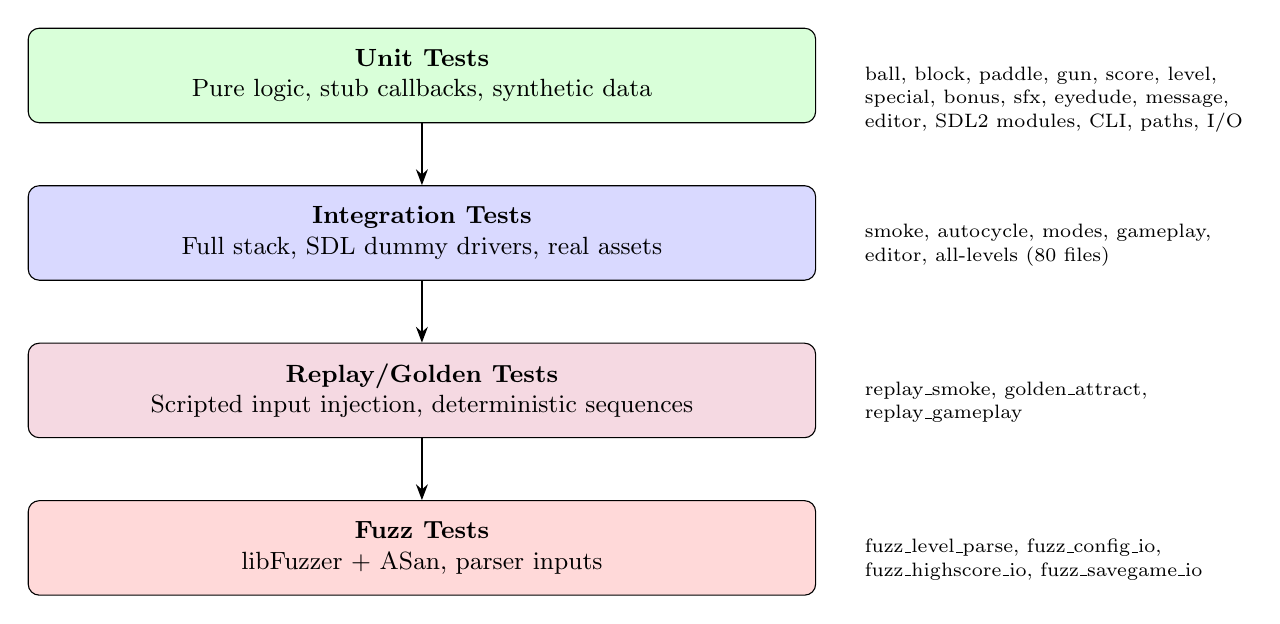
\begin{tikzpicture}[
    layer/.style={draw, rounded corners, minimum width=10cm, minimum height=1.2cm, font=\small, align=center},
    arrow/.style={-{Stealth[length=2mm]}, thick},
]
\node[layer, fill=green!15] (unit) at (0, 0) {\textbf{Unit Tests}\\Pure logic, stub callbacks, synthetic data};
\node[layer, fill=blue!15] (integ) at (0, -2) {\textbf{Integration Tests}\\Full stack, SDL dummy drivers, real assets};
\node[layer, fill=purple!15] (replay) at (0, -4) {\textbf{Replay/Golden Tests}\\Scripted input injection, deterministic sequences};
\node[layer, fill=red!15] (fuzz) at (0, -6) {\textbf{Fuzz Tests}\\libFuzzer + ASan, parser inputs};

\draw[arrow] (unit) -- (integ);
\draw[arrow] (integ) -- (replay);
\draw[arrow] (replay) -- (fuzz);

\node[font=\scriptsize, anchor=west] at (5.5, 0) {ball, block, paddle, gun, score, level,};
\node[font=\scriptsize, anchor=west] at (5.5, -0.3) {special, bonus, sfx, eyedude, message,};
\node[font=\scriptsize, anchor=west] at (5.5, -0.6) {editor, SDL2 modules, CLI, paths, I/O};

\node[font=\scriptsize, anchor=west] at (5.5, -2) {smoke, autocycle, modes, gameplay,};
\node[font=\scriptsize, anchor=west] at (5.5, -2.3) {editor, all-levels (80 files)};

\node[font=\scriptsize, anchor=west] at (5.5, -4) {replay\_smoke, golden\_attract,};
\node[font=\scriptsize, anchor=west] at (5.5, -4.3) {replay\_gameplay};

\node[font=\scriptsize, anchor=west] at (5.5, -6) {fuzz\_level\_parse, fuzz\_config\_io,};
\node[font=\scriptsize, anchor=west] at (5.5, -6.3) {fuzz\_highscore\_io, fuzz\_savegame\_io};

\end{tikzpicture}
\caption{Test infrastructure layers. Each layer builds on the one below. Unit tests cover individual modules; integration tests exercise the full stack.}
\label{fig:test-layers}
\end{figure}

\subsection{Headless Testing}
\label{sec:headless}

SDL2 dummy drivers enable CI testing without display or audio hardware:
\begin{lstlisting}[language={}, numbers=none, frame=none]
SDL_VIDEODRIVER=dummy    # No window created, textures still allocate
SDL_AUDIODRIVER=dummy    # Mix_OpenAudio succeeds silently
\end{lstlisting}

\subsection{Sanitizer Builds}
\label{sec:sanitizers}

The \code{asan} preset builds all targets with \code{-fsanitize=address,undefined -fno-omit-frame-pointer}. Both debug and sanitizer configurations run in CI on every push and PR.

\subsection{Fuzz Testing}
\label{sec:fuzz}

Four libFuzzer harnesses target parser inputs (Clang only):
\begin{description}[nosep, leftmargin=2em]
    \item[fuzz\_level\_parse] Level file parser (character mapping, title/time parsing)
    \item[fuzz\_config\_io] TOML config parser
    \item[fuzz\_highscore\_io] JSON high score parser
    \item[fuzz\_savegame\_io] JSON save game parser
\end{description}

Not registered as ctest targets (they run indefinitely). Manually invoked: \code{./build/tests/fuzz\_level\_parse -max\_total\_time=30}.

\subsection{Integration Test Categories}
\label{sec:integ-tests}

\begin{table}[h]
\centering
\caption{Integration test suite}
\label{tab:integ-tests}
\begin{tabularx}{\textwidth}{lX}
\toprule
\textbf{Test} & \textbf{Scope} \\
\midrule
\code{test\_integration\_smoke} & Full \funcname{game\_create}/\funcname{game\_destroy} lifecycle \\
\code{test\_integration\_autocycle} & Attract sequence: PRESENTS$\rightarrow$INTRO$\rightarrow$...$\rightarrow$HIGHSCORE$\rightarrow$INTRO \\
\code{test\_integration\_modes} & Force-transition to each of 12 modes, tick N frames, verify no crashes \\
\code{test\_integration\_gameplay} & Enter GAME mode, verify state, block loading, ball/paddle, extended ticking \\
\code{test\_integration\_editor} & Enter EDIT mode, draw blocks, clear, play-test transitions \\
\code{test\_replay\_smoke} & Synthetic key injection, scripted mode transitions \\
\code{test\_golden\_attract} & Deterministic attract cycle mode transitions and timing \\
\code{test\_replay\_gameplay} & Scripted gameplay: start, paddle, shoot, pause, extended play \\
\code{test\_integration\_all\_levels} & Load all 80 levels, verify parse, tick 100 frames each (120s timeout) \\
\bottomrule
\end{tabularx}
\end{table}


% =============================================================================
\section{CI/CD}
\label{sec:cicd}
% =============================================================================

Three GitHub Actions workflows run on every push to \code{master} and every PR.

\begin{figure}[h]
\centering
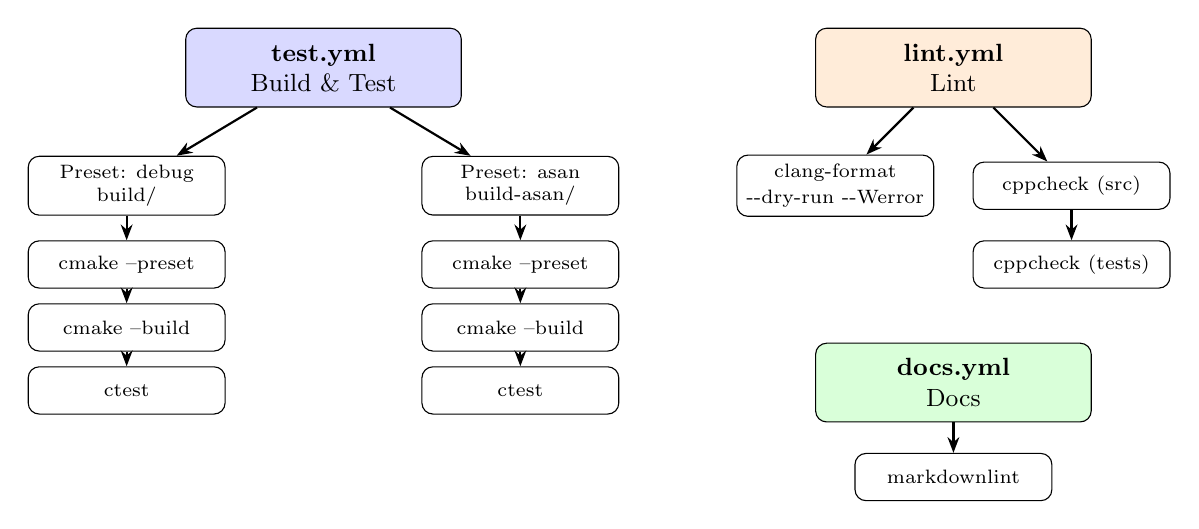
\begin{tikzpicture}[
    job/.style={draw, rounded corners, fill=#1, minimum width=3.5cm, minimum height=1cm, font=\small, align=center},
    pipestep/.style={draw, rounded corners, fill=white, minimum width=2.5cm, minimum height=0.6cm, font=\scriptsize, align=center},
    arrow/.style={-{Stealth[length=2mm]}, thick},
]

% test.yml
\node[job=blue!15] (test) at (0, 0) {\textbf{test.yml}\\Build \& Test};
\node[pipestep] (debug) at (-2.5, -1.5) {Preset: debug\\build/};
\node[pipestep] (asan) at (2.5, -1.5) {Preset: asan\\build-asan/};
\node[pipestep] (conf1) at (-2.5, -2.5) {cmake --preset};
\node[pipestep] (build1) at (-2.5, -3.3) {cmake --build};
\node[pipestep] (ctest1) at (-2.5, -4.1) {ctest};
\node[pipestep] (conf2) at (2.5, -2.5) {cmake --preset};
\node[pipestep] (build2) at (2.5, -3.3) {cmake --build};
\node[pipestep] (ctest2) at (2.5, -4.1) {ctest};

\draw[arrow] (test) -- (debug);
\draw[arrow] (test) -- (asan);
\draw[arrow] (debug) -- (conf1);
\draw[arrow] (conf1) -- (build1);
\draw[arrow] (build1) -- (ctest1);
\draw[arrow] (asan) -- (conf2);
\draw[arrow] (conf2) -- (build2);
\draw[arrow] (build2) -- (ctest2);

% lint.yml
\node[job=orange!15] (lint) at (8, 0) {\textbf{lint.yml}\\Lint};
\node[pipestep] (fmt) at (6.5, -1.5) {\shortstack{clang-format\\{-}{-}dry-run {-}{-}Werror}};
\node[pipestep] (cpp1) at (9.5, -1.5) {cppcheck (src)};
\node[pipestep] (cpp2) at (9.5, -2.5) {cppcheck (tests)};

\draw[arrow] (lint) -- (fmt);
\draw[arrow] (lint) -- (cpp1);
\draw[arrow] (cpp1) -- (cpp2);

% docs.yml
\node[job=green!15] (docs) at (8, -4) {\textbf{docs.yml}\\Docs};
\node[pipestep] (mdlint) at (8, -5.2) {markdownlint};
\draw[arrow] (docs) -- (mdlint);

\end{tikzpicture}
\caption{CI pipeline. Build matrix runs Debug and ASan configurations in parallel. Lint checks clang-format and cppcheck. Docs checks markdown.}
\label{fig:ci-pipeline}
\end{figure}

\begin{table}[h]
\centering
\caption{CI workflow details}
\label{tab:ci-workflows}
\begin{tabularx}{\textwidth}{llX}
\toprule
\textbf{Workflow} & \textbf{Jobs} & \textbf{Checks} \\
\midrule
\code{test.yml} & 2 (matrix) & Configure, build, run all ctest targets. Fail-fast disabled. \\
\code{lint.yml} & 2 & clang-format \code{src/*.c include/*.h}; cppcheck \code{src/} and \code{tests/} with warning, style, performance, portability. \\
\code{docs.yml} & 1 & markdownlint on all \code{.md} files. \\
\bottomrule
\end{tabularx}
\end{table}


% =============================================================================
\section{Module Dependency Map}
\label{sec:dep-map}
% =============================================================================

\begin{figure}[h]
\centering
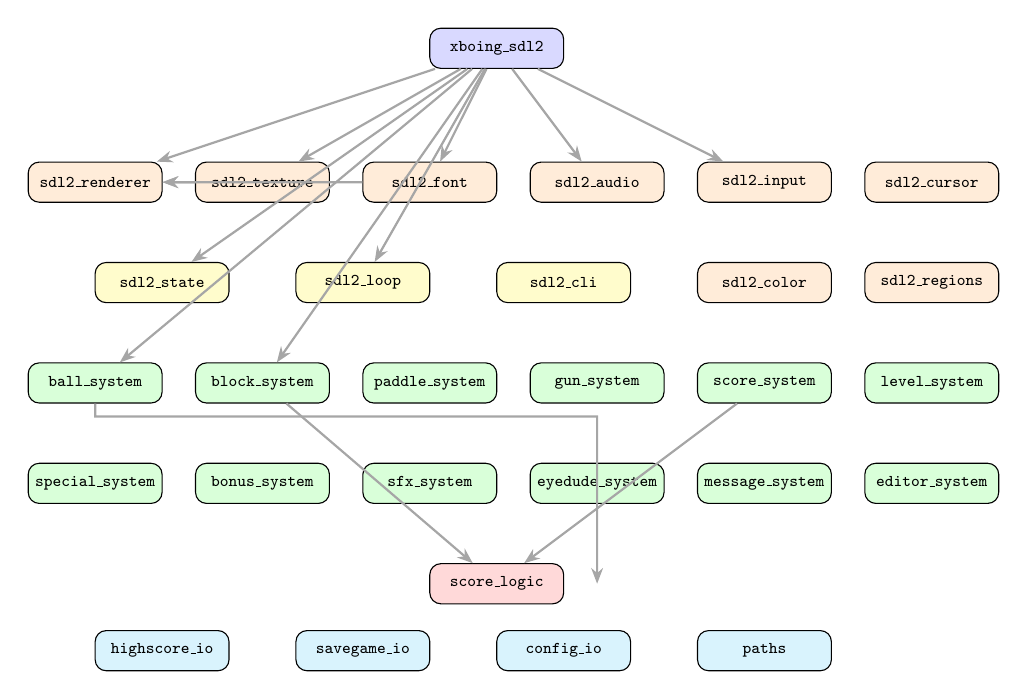
\begin{tikzpicture}[
    mod/.style={draw, rounded corners, fill=#1, minimum width=2cm, minimum height=0.6cm, font=\scriptsize\ttfamily, inner sep=2pt},
    dep/.style={-{Stealth[length=2mm]}, thick, gray!70},
    scale=0.85, transform shape,
]

% Integration layer
\node[mod=blue!15] (exe) at (0, 8) {xboing\_sdl2};

% SDL2 platform row
\node[mod=orange!15] (rend) at (-6, 6) {sdl2\_renderer};
\node[mod=orange!15] (tex) at (-3.5, 6) {sdl2\_texture};
\node[mod=orange!15] (fnt) at (-1, 6) {sdl2\_font};
\node[mod=orange!15] (aud) at (1.5, 6) {sdl2\_audio};
\node[mod=orange!15] (inp) at (4, 6) {sdl2\_input};
\node[mod=orange!15] (cur) at (6.5, 6) {sdl2\_cursor};

% Pure C engine row
\node[mod=yellow!20] (sta) at (-5, 4.5) {sdl2\_state};
\node[mod=yellow!20] (lop) at (-2, 4.5) {sdl2\_loop};
\node[mod=yellow!20] (cli) at (1, 4.5) {sdl2\_cli};
\node[mod=orange!15] (col) at (4, 4.5) {sdl2\_color};
\node[mod=orange!15] (reg) at (6.5, 4.5) {sdl2\_regions};

% Game systems row
\node[mod=green!15] (ball) at (-6, 3) {ball\_system};
\node[mod=green!15] (blk) at (-3.5, 3) {block\_system};
\node[mod=green!15] (pad) at (-1, 3) {paddle\_system};
\node[mod=green!15] (gun) at (1.5, 3) {gun\_system};
\node[mod=green!15] (scr) at (4, 3) {score\_system};
\node[mod=green!15] (lvl) at (6.5, 3) {level\_system};

\node[mod=green!15] (spc) at (-6, 1.5) {special\_system};
\node[mod=green!15] (bon) at (-3.5, 1.5) {bonus\_system};
\node[mod=green!15] (sfx) at (-1, 1.5) {sfx\_system};
\node[mod=green!15] (eye) at (1.5, 1.5) {eyedude\_system};
\node[mod=green!15] (msg) at (4, 1.5) {message\_system};
\node[mod=green!15] (edt) at (6.5, 1.5) {editor\_system};

% Shared arithmetic
\node[mod=red!15] (slg) at (0, 0) {score\_logic};

% Persistence row
\node[mod=cyan!15] (hio) at (-5, -1) {highscore\_io};
\node[mod=cyan!15] (sio) at (-2, -1) {savegame\_io};
\node[mod=cyan!15] (cio) at (1, -1) {config\_io};
\node[mod=cyan!15] (pth) at (4, -1) {paths};

% Key dependencies
\draw[dep] (exe) -- (rend);
\draw[dep] (exe) -- (tex);
\draw[dep] (exe) -- (fnt);
\draw[dep] (exe) -- (aud);
\draw[dep] (exe) -- (inp);
\draw[dep] (exe) -- (ball);
\draw[dep] (exe) -- (blk);
\draw[dep] (exe) -- (sta);
\draw[dep] (exe) -- (lop);

\draw[dep] (tex) -- (rend);
\draw[dep] (fnt) -- (rend);

\draw[dep] (blk) -- (slg);
\draw[dep] (scr) -- (slg);

\draw[dep] (ball) -- ++(0,-0.5) -| ($(slg)+(1.5,0.5)$) -- ($(slg)+(1.5,0)$);

\end{tikzpicture}
\caption{Module dependency graph. The executable links all libraries. \modulename{score\_logic} is the only shared dependency between game systems (\modulename{block\_system} for hit points, \modulename{score\_system} for multiplier/threshold). \modulename{sdl2\_texture} and \modulename{sdl2\_font} depend on \modulename{sdl2\_renderer} for the \code{SDL\_Renderer*} handle.}
\label{fig:dep-map}
\end{figure}


% =============================================================================
\section{Legacy Comparison}
\label{sec:legacy-compare}
% =============================================================================

\begin{table}[h]
\centering
\caption{Structural comparison with legacy codebase}
\label{tab:legacy-compare}
\begin{tabularx}{\textwidth}{Xll}
\toprule
\textbf{Aspect} & \textbf{Legacy} & \textbf{Modern} \\
\midrule
Global mutable variables & 50+ & 0 \\
X11/platform API calls in game logic & $\sim$800 & 0 (in system libs) \\
Audio drivers & 12 (platform-specific) & 1 (SDL2\_mixer) \\
Build system & Makefile & CMake with presets \\
Static library decomposition & none & per-module \\
Test suite & none & unit, integration, replay, fuzz \\
CI & none & build + lint + docs \\
\bottomrule
\end{tabularx}
\end{table}

The modern codebase is larger in source LOC than legacy, reflecting the modular structure (function signatures, opaque context boilerplate, callback table definitions) and comprehensive error handling. The test suite exceeds the source in LOC.


% =============================================================================
\section{Architectural Decision Records Summary}
\label{sec:adrs}
% =============================================================================

All ADRs are recorded in \filename{docs/DESIGN.md}. \Cref{tab:adrs} summarizes each with status and key rationale.

\begin{longtable}{lllp{7cm}}
\caption{Architectural Decision Records} \label{tab:adrs} \\
\toprule
\textbf{ADR} & \textbf{Status} & \textbf{Module} & \textbf{Key Rationale} \\
\midrule
\endfirsthead
\toprule
\textbf{ADR} & \textbf{Status} & \textbf{Module} & \textbf{Key Rationale} \\
\midrule
\endhead
\bottomrule
\endfoot

001 & Accepted & Build & CMake as sole build system; no Meson. Existing CI and presets carry forward. \\
002 & Accepted & paths & XDG Base Directory resolution. Centralizes 12+ scattered callsites. Caller-provided buffers. \\
003 & Accepted & CMake & FHS-compliant install targets. Dev mode unchanged (relative paths). \\
004 & Accepted & sdl2\_renderer & Single window, 575$\times$720 logical resolution, 2$\times$ scale, GPU-accelerated, nearest-neighbor. \\
005 & Accepted & sdl2\_texture & FNV-1a hash map, eager PNG loading, 256 slots, partial load tolerance. \\
006 & Accepted & sdl2\_font & 4 Liberation Sans TTF fonts, transient textures, 2px shadow offset. \\
007 & Accepted & sdl2\_color & Static const RGBA, X11 rgb.txt verified, 7-step gradients. No opaque context. \\
008 & Accepted & sdl2\_cursor & Pre-created cursors, best-effort, visibility toggle for NONE. \\
009 & Accepted & sdl2\_regions & 9 named SDL\_Rect constants replacing X11 sub-windows. No opaque context. \\
010 & Accepted & sdl2\_audio & SDL2\_mixer, eager WAV caching, FNV-1a hash map, 16 concurrent channels. \\
011 & Accepted & sdl2\_input & Scancode-to-action mapping, dual bindings, level+edge triggers, runtime rebindable. \\
012 & Accepted & sdl2\_state & Function pointer dispatch, enter/update/exit hooks, dialogue push/pop. Pure C. \\
013 & Accepted & sdl2\_loop & Fixed-timestep accumulator, microsecond precision, spiral-of-death prevention. Pure C. \\
014 & Accepted & sdl2\_cli & Config struct pattern, exact match, status code return. Pure C. \\
015 & Accepted & ball\_system & Callback table (7 ptrs), environment struct (12 fields), preserves known bugs. \\
016 & Accepted & block\_system & Diagonal cross-product collision replacing X11 Regions. Adjacency filter. \\
017 & Accepted & paddle\_system & Position, size, reverse, delta tracking. Mouse formula preserved. \\
018 & Accepted & gun\_system & 40 bullet slots, 40 tink slots, 8 callbacks, collision priority preserved. \\
019 & Accepted & score\_system & Reuses score\_logic, digit layout, x2-wins-over-x4 bug preserved. \\
020 & Accepted & level\_system & Single callback, 30-char mapping, level wrapping, background cycling. \\
021 & Accepted & special\_system & 8 specials (7 managed, 1 paddle-owned), mutual exclusion (x2/x4), saving persistence. \\
022 & Accepted & bonus\_system & 10-state tally, score pre-commit, save trigger every 5 levels. \\
023 & Accepted & sfx\_system & 5 effects + BorderGlow, query-based rendering, injectable random. \\
024 & Accepted & eyedude\_system & 6 walk frames, AABB collision, 10{,}000 point bonus, injectable random. \\
025 & Accepted & presents\_system & 14-state sequencer, unified typewriter, sound events as data. \\
026 & Accepted & intro\_system & 2 modes (intro+instruct), static data tables, shared sparkle. \\
027 & Accepted & demo\_system & 2 modes (demo+preview), ball trail data, level loading callback. \\
028 & Accepted & keys\_system & 2 modes (game+editor), static key binding tables, blink timing. \\
029 & Accepted & dialogue\_system & Modal input with 4 validation modes (text, numeric, printable, yes/no). \\
030 & Accepted & highscore\_system & Title sparkle, row sparkle, specials timing, score display. \\
031 & Accepted & message\_system & Single-line message bar with auto-clear delay. \\
032 & Accepted & highscore\_io & JSON format replacing legacy binary. Hand-written parser, atomic writes. \\
033 & Accepted & savegame\_io & JSON format replacing legacy binary. Level, score, lives, specials, grid snapshot. \\
034 & Accepted & config\_io & Minimal TOML format. User preferences persisted at XDG data path. \\
035 & Accepted & cppcheck & cppcheck pass across entire codebase. \\
036 & Accepted & clang-tidy & clang-tidy pass with \filename{.clang-tidy} configuration. \\
037 & Accepted & paths & Asset directory resolution for installed binaries. \\

\end{longtable}


% =============================================================================
\section{Glossary}
\label{sec:glossary}
% =============================================================================

\begin{description}[nosep, leftmargin=3em]
    \item[Legacy] The original X11/Xlib codebase (1993--1996, \filename{original/} directory).
    \item[Modern] The SDL2-based codebase (\filename{src/}, \filename{include/}).
    \item[Opaque context] Heap-allocated struct hidden behind a forward-declared typedef; accessed only via public API functions.
    \item[Callback injection] Providing function pointer tables at module creation time so the module can communicate side effects without direct dependencies on other modules.
    \item[Environment struct] A const struct carrying per-frame state from other systems, passed to update functions. Replaces extern globals.
    \item[FNV-1a] Fowler--Noll--Vo hash function variant 1a; used for texture and audio cache hash maps.
    \item[XDG] X Desktop Group Base Directory Specification; standard Linux paths for user data, config, and cache.
    \item[FHS] Filesystem Hierarchy Standard; standard Linux install paths (\code{/usr/share/}, \code{/usr/bin/}).
    \item[Sequencer] A UI module that advances through a state machine per frame, exposing render data through query functions. Does not render directly.
\end{description}

\end{document}
